\section{Rolling Memory Erases What Is Said Once}
\label{sec:findings}

% OUTLINE with current numbers (docs/pilot_findings.md); final tables/figures TODO.

\paragraph{Main result.}
\begin{figure}[t]
\centering
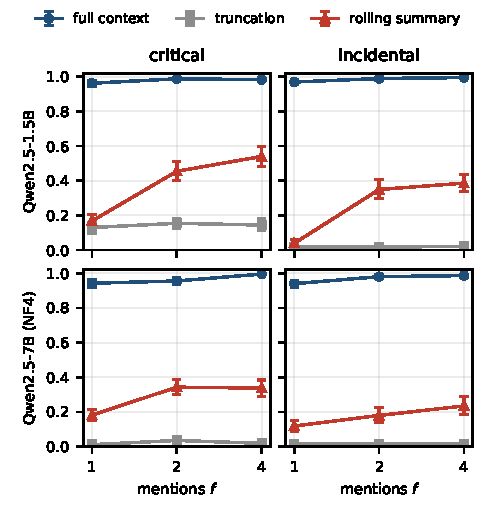
\includegraphics[width=\columnwidth]{figures/retention.pdf}
\caption{Accuracy after a claim's last mention as a function of how often it was mentioned ($B{=}160$, pooled over four domains). Full context is flat in $f$; the rolling summary keeps what was repeated. Truncation keeps only the most recent text and is flat as well. Bars: 95\% dialogue-clustered bootstrap CIs.}
\label{fig:retention}
\end{figure}
\begin{itemize}
\item Qwen2.5-1.5B, four domains, $B{=}160$: full-context slope $+0.006$ to $+0.013$; rolling slope $+0.16$ to $+0.27$; $\delta$ significant in every domain for both critical and incidental claims (e.g.\ critical: Heron $+0.27$, city $+0.10$, science $+0.15$, product $+0.19$, all $p\le .002$). Single-mention critical claims keep 4--22\% of full-context accuracy, four-mention ones 36--75\%.
\item Qwen2.5-7B: $\delta_{\text{crit}}=+0.105$ on Heron ($p=.002$), weaker pooled over the other three domains ($+0.034$, $p=.03$).
\item Gemma-4-E4B: importance-driven retention; $\delta$ significant only at $B{=}80$ for critical claims (city $+0.081$, science $+0.120$), not on product.
\item Phi-3.5-mini: erases most claims regardless of frequency; no summarisation-specific slope.
\end{itemize}

\paragraph{Controls.}
Truncation is flat in frequency, so the effect is not recency. Empty memory: 0--19\% (guessing floor).
Clustered schedule (mentions in the $f$ sessions ending at $L$, so repeated claims are not introduced earlier): $\beta_{\log f}$ stays positive and significant for Qwen-1.5B and Phi-3.5 \todo{DiD version}.

\paragraph{Budget.}
At $B{=}80$ rolling erases nearly everything for small models, so the frequency gradient is compressed; the gradient is clearest at $B{=}160$, where there is room to keep something and the summariser chooses what was repeated.

\paragraph{A second failure: wholesale overwrite.}
On product at $B{=}160$, Gemma writes notes for the newest meeting only, keeping ${\sim}6\%$ of claims at every frequency. We report this frequency-independent failure separately.

\paragraph{The writer, not the reader.}
If small models were merely poor at reading notes, the frequency gradient could come from the reader.
We re-probe every writer's Heron memories with one fixed reader (Qwen2.5-7B, NF4) and compare with the same reader's full-context probes.
The gradient is a property of the memory: Qwen-1.5B memories read by the 7B reader give $\delta_{\text{crit}}=+0.255$ at $B{=}160$ ($p<10^{-13}$; self-read: $+0.272$), with single-mention critical claims keeping 5\% of full-context accuracy against 64\% at $f{=}4$; incidental $+0.198$.
Phi-3.5 memories show a weaker gradient (incidental $+0.101$, $p=.005$; critical $+0.044$ to $+0.061$, $p\ge.06$), and Gemma memories none ($|\delta|\le0.016$), matching their self-read profiles.

\paragraph{Naturalistic dialogues.}
Templated lines could make repeated claims easy to spot.
We therefore had an LLM rewrite every session of the Heron and city dialogues into free-flowing meeting talk, under checks that each claim's key facts survive, and re-ran Qwen-1.5B.
Full context stays flat in frequency (slopes $\le+0.008$), and rolling memory again rewards repetition: at $B{=}160$, $\delta_{\text{crit}}=+0.218$ on Heron ($p<10^{-11}$; templated $+0.27$) and $+0.062$ on city ($p=.047$; templated $+0.10$), pooled $+0.140$ ($p<10^{-8}$).
Single-mention critical claims keep 17\% of full-context accuracy, four-mention ones 46\%.
On city, rolling memory over the naturalised text erases almost all incidental claims (5--12\% at every frequency), which leaves no gradient to measure.

\paragraph{From recall to decisions.}
Recognising a claim is not the same as acting on it.
For each critical claim we wrote a decision question that puts the agent in front of the choice the claim bears on (\emph{``The team plans to wipe the old servers and rely on the nightly backup. What should they do first?''}), with four options: the action that applies the claim, a lure that proceeds as if the claim had never been raised, an action built on a wrong detail, and ``not mentioned''.
With the full transcript both models choose the right action 91--99\% of the time.
Under rolling memory at $B{=}160$, a single-mention claim leads to the right action only 34\% (Qwen-1.5B) and 16\% (Qwen-7B) of the time, and the frequency gradient carries over to decisions ($\delta=+0.079$, $p<10^{-5}$, and $+0.052$, $p<.001$, pooled over four domains).
The two models fail differently.
Qwen-1.5B takes the lure in 15\% of single-mention cases against 2\% with full context, proceeding as planned past a warning it has forgotten.
Qwen-7B never takes the lure; it answers that the notes are silent (83\%), which is safer but still leaves the decision unmade.
